

% -------------------------------------------------------

\section{String Resonances}
\label{appString}

String theory is believed to encompass an enormous landscape of solutions.
Among these are a rather naturally appearing subclass with large internal
volume and a fundamental string scale not too far above the electroweak
scale.
If this possibility is realized in nature, then the LHC may provide
a direct probe of string scale physics.
One definitive prediction of string theory is that
scattering amplitudes are modified in interesting ways
near the string scale.
For experiments at the LHC, the most spectacular such modification
would be the appearance of dijet resonances
corresponding to excited string states~\cite{Cullen:2000ef,Anchordoqui:2008di}.

The leading order $2 \rightarrow 2$ Veneziano scattering amplitudes in any
string theory may be represented
as field theory amplitudes
modified by a universal form factor
%that represents
%the exchange of an infinite tower of string Regge excitations
in the appropriate kinematic channels~\cite{Cullen:2000ef}.
The Veneziano form factor as a function of Mandelstam variables
$V(x,y) = \widehat{V}(\alpha' x, \alpha' y)$, where
$(x,y) \in (s,t,u)$ and
$\alpha'=1/m_s^2$ and $m_s$ is the string scale,
may be written
in terms of gamma functions as
\begin{equation}
\widehat{V}(x,y) = {  \Gamma(1-x) \Gamma(1-y) \over
\Gamma(1-x-y) }
\end{equation}
It satisfies crossing symmetry
$\widehat{V}(x,y) = \widehat{V}(y,x)$,
and has the limit
\begin{equation}
\lim_{x,y \to 0} \widehat{V}(x,y) = 1
\end{equation}
The Veneziano form factor
may be represented as a  sum over an infinite tower of
Regge excitations in the $x$-channel as
\begin{eqnarray}
\widehat{V}(x,y) &=& {x \over x+y} \sum_{n=0}^{\infty} {1 \over n !  (x-n) }
 \prod_{j=0}^n (y+j)  \nonumber \\
&=& {x \over x+y} \sum_{n=0}^{\infty} {1 \over n !  (x-n) }
 \sum_{j=0}^{n} |s(n+1,j+1)| y^{j+1}
 \label{reggesum}
\end{eqnarray}
where $s(n+1,j+1)$ are the Stirling numbers of the first kind.
The
Regge excitations in the sum (\ref{reggesum})
have the same  gauge and global quantum numbers
as massless particles of spin $J_0$ that can be exchanged
in the $x$-channel, but
with masses squared $m_n^2 = n m_s^2$ for
$n=1,2,\dots, \infty$ and spins at each level $n$ given
by $J_{n,j} = J_0 + j$ where $j=0, \dots, n$.


The first Regge excitations at level $n=1$
include excited gluons
$g_{1,1}^*$ and $g_{1,2}^*$ of spin $J=1,2$,
and excited quarks $q_{1,{1\over 2},i}^*$ and
$q_{1,{3\over 2},i}^*$ of spin $J={1\over 2},{3\over 2}$
for each quark species $i$,
all with masses equal (up to small finite corrections)
to the string scale.
For $s$-channel scattering at a hadron collider, all
these excitations contribute to produce  a dijet resonance
at the string scale.



% ---------

% -----



The specific form of $2 \rightarrow 2$ string scattering amplitudes
may depend on details of the string theory model.
However, there are certain model-independent features that follow
from Regge excitations that must exist in certain channels in
any realization of string theory at the TeV scale.
The only such model-independent Regge excitations that
are included here
are in channels that have the same flavor quantum numbers
as those of massless particles
in the Standard Model.
With this restriction, the matrix elements
for all strongly interacting $2 \rightarrow 2$ parton
level scattering processes
that are modified by Veneziano form factors in the appropriate channels
are
\begin{eqnarray}
{\mathcal M}(g^{\pm}_a g^{\pm}_b \rightarrow g^{\pm}_c g^{\pm}_d) &=& g^2
    \frac{s^2}{stu}  \Bigg[  2 sV(t,u) ~{\bf P}^{~~~ab}_{\! {\bf 27}~cd}
    +3\left(tV(s,u)-uV(s,t)\right) {\bf P}_{{\bf 8_A}~cd}^{~~ab}
  \nonumber \\
  &+&\frac{5}{3}\left(tV(s,u)+uV(s,t)-\frac{4}{5}sV(t,u)\right)
   {\bf P}_{{\bf 8_S}~cd}^{~~ab}
  \nonumber\\
  &+&\frac{16}{3}\left(tV(s,u)+uV(s,t)-\frac{1}{8}sV(t,u)\right)
  {\bf P}_{{\bf 1}~cd}^{~~ab}
   \Bigg]  \\
{\mathcal M}(g^{\pm}_a g^{\mp}_b \rightarrow g^{\pm}_c g^{\mp}_d )  &=& g^2
    \frac{u^2}{stu} \Bigg[  2sV(t,u) ~{\bf P}^{~~~ab}_{\! {\bf 27}~cd}
    +3\left(tV(s,u)-uV(s,t)\right)
     {\bf P}_{{\bf 8_A}~cd}^{~~ab}
    \nonumber\\
  &+&\frac{5}{3}\left(tV(s,u)+uV(s,t)-\frac{4}{5}sV(t,u)\right)
    {\bf P}_{{\bf 8_S}~cd}^{~~ab}
    \nonumber\\
  &+&\frac{16}{3}\left(tV(s,u)+uV(s,t)-\frac{1}{8}sV(t,u)\right)
   {\bf P}_{ {\bf 1}~cd}^{~~ab}
  \Bigg]  \\
{\mathcal M}(g^{\pm}_a g^{\mp}_b \rightarrow g^{\mp}_c g^{\pm}_d)   &=& g^2
  \frac{t^2}{stu} \Bigg[ 2sV(t,u) ~{\bf P}^{~~~ab}_{\! {\bf 27}~cd}
    +3\left(tV(s,u)-uV(s,t)\right)
    {\bf P}_{{\bf 8_A}~cd}^{~~ab}
   \nonumber\\
  &+&\frac{5}{3}\left(tV(s,u)+uV(s,t)-\frac{4}{5}sV(t,u)\right)
  {\bf P}_{{\bf 8_S}~cd}^{~~ab}
   \nonumber\\
  &+&\frac{16}{3}\left(tV(s,u)+uV(s,t)-\frac{1}{8}sV(t,u)\right)
  {\bf P}_{{\bf 1}~cd}^{~~ab}
  \Bigg]
  \\
%
%
%\begin{eqnarray}
{\mathcal M} (g_a^{\pm}g_b^{\mp} \to  \overline{q}_{\bar{i}}^{\mp}  q_j^{\pm})    &=& g^2
   \frac{u}{s}  \Bigg[
      \bigg( \sqrt{\frac{u}{t}}V(s,t)+\sqrt{\frac{t}{u}}V(s,u) \bigg)
     \bigg( \sqrt{\frac{5}{6}}  ~{\bf P}_{{\bf 8_S}~\bar{i} j }^{~~ab}
       +\sqrt{\frac{8}{3}}   ~{\bf P}_{{\bf 1}~\bar{i} j }^{~~ab}    \bigg)
       \nonumber \\
   &+&  \bigg(  \sqrt{\frac{u}{t}} V(s,t)-\sqrt{\frac{t}{u}}V(s,u) \bigg) \sqrt{\frac{3}{2}}
        ~{\bf P}_{{\bf 8_A}~\bar{i} j }^{~~ab}
   \Bigg] \\
{\mathcal M} (g_a^{\pm}g_b^{\mp} \to \overline{q}_{\bar{i}}^{\pm}  q_j^{\mp}   )    &=& g^2
   \frac{t}{s} \Bigg[
     \bigg(  \sqrt{\frac{u}{t}}V(s,t)+\sqrt{\frac{t}{u}}V(s,u)  \bigg)
     \bigg(  \sqrt{\frac{5}{6}}  ~{\bf P}_{{\bf 8_S}~\bar{i} j }^{~~ab}
      +\sqrt{\frac{8}{3}}   ~{\bf P}_{{\bf 1}~\bar{i} j }^{~~ab}      \bigg)
     \nonumber \\
   &+& \bigg(  \sqrt{ \frac{u}{t}}V(s,t)-\sqrt{\frac{t}{u}}V(s,u)  \bigg)  \sqrt{\frac{3}{2}}
    ~{\bf P}_{{\bf 8_A}~\bar{i} j }^{~~ab}
     \Bigg]
  \\
%\end{eqnarray}
%
%
%\begin{eqnarray}
{\mathcal M} (q_i^{\pm}g_a^{\pm} \to q_j^{\pm} g_b^{\pm} )   &=& g^2
   \frac{s}{t} \Bigg[  \sqrt{-\frac{u}{s}}V(s,t)(
 ~{\bf P}_{{\bf 15}~bj}^{~~~ai}
   -
  ~{\bf P}_{\bar{\bf 6}~bj}^{~~ai}
   )
   \nonumber\\
   &-&\frac{1}{3}\left(\sqrt{-\frac{u}{s}}V(s,t)+8\sqrt{-\frac{s}{u}}V(t,u)\right)
   {\bf P}_{{\bf 3}~bj}^{~~ai}
    \Bigg]
    \\
{\mathcal M} (q_i^{\pm}g_a^{\mp} \to q_j^{\pm} g_b^{\mp})  &=& g^2
   \frac{u}{t}\Bigg[
     \sqrt{-\frac{u}{s}}V(s,t)(
 ~{\bf P}_{{\bf 15}~bj}^{~~~ai}
   -
  ~{\bf P}_{\bar{\bf 6}~bj}^{~~ai}
     )
      \nonumber \\
   &-&\frac{1}{3}\left(\sqrt{-\frac{u}{s}}V(s,t)+8\sqrt{-\frac{s}{u}}V(t,u)\right)
    {\bf P}_{{\bf 3}~bj}^{~~ai}
      \Bigg]
      \\
%\end{eqnarray}
%
%
%\begin{eqnarray}
{\mathcal M}  (q_i^{\pm}\overline{q}^{\mp}_{\bar{j}} \to q_k^{\pm}\overline{q}^{\mp}_{\bar{\ell}} )
      &=& g^2
    \Bigg[ \left(\frac{u}{s}-\frac{u}{3t}\right)
   {\bf P}_{{\bf 8}~k \bar{\ell} }^{~~i \bar{j}}
 +   {8 u \over 3 t} ~{\bf P}_{{\bf 1}~k \bar{\ell} }^{~~i \bar{j}}
    \Bigg] V(s,t)
% \\
\end{eqnarray}
where the ${\bf P}^{\alpha \beta}_{~\gamma \delta} $
tensors are projection operators between irreducible
$SU(3)_C$ representations in the initial and final states.
Matrix elements related to these by charge conjugation or time reversal are not
shown.
The inclusion of only this minimal set of stringy modifications of
the scattering amplitudes allows
the results of the dijet
resonance search to be presented as
a model-independent probe of the string scale.
In specific models there may be additional Regge resonances
in other channels that could increase the strength of
dijet resonances somewhat.

For the dijet resonance search, the main interest is in the
total cross section of the first $s$-channel Regge resonance in the narrow
width limit.
The resonant matrix elements squared in this limit may be obtained from
the ones given above by replacing
the propagator factor of
any Veneziano form factor that involves the $s$-channel
with a Breit-Wigner form in that channel for $n=1$ only, and by ignoring
any interference between the $s$ and $t$ or $u$ channels.
In this limit, all Veneziano
form factors in the matrix element squared
may then be neglected except for the squares of ones that involve
the $s$-channel
\begin{equation}
{ |V(s,y)|^2 \over y^2} \simeq {1 \over (s - m_s^2)^2 + m_s^2 \Gamma^2 }
\label{V-BW}
\end{equation}
where $y \in (t,u)$ and
$\Gamma \equiv \Gamma({\rm Initial} \to R^{(1)} \to {\rm All})$
is the total width of the coherent superposition of
$n=1$ Regge excitations arising from the appropriate initial state parton scattering
channel.


Using the optical theorem
the widths of the $n=1$ Regge excitations  in a given channel
may be obtained from the
residue of the leading order (ignoring the finite width)
total cross sections near the $n=1$ $s$-channel pole after dividing
by the wave function factor for the external states
obtained from the residue of the forward scattering amplitude
\begin{equation}
{1 \over m_s} \Gamma({\rm Initial} \to R^{(1)} \to {\rm All}) =
  m_s^2 ~
{ {\rm Res}_2 [ \sigma( {\rm Initial} \to R^{(1)} \to{\rm All} ) ]
  \over
    {\rm Res}_1 [ {\cal M}({\rm Initial} \to {\rm Initial}) ] }
\end{equation}
where ${\rm Res}_k [f(s)] = f(s) (s - m_s^2)^k$ extracts $s$-channel
the pole(s).
Using this relation and matrix elements
given above, the decay total widths on the first Regge excitations
for all non-trivial initial state helicity and color
configurations in $2 \to 2$ QCD scattering on these resonances are
\begin{eqnarray}
{1 \over m_s}  \Gamma (q_i^{\pm} g_a^{\pm} \to R^{(1)} \to
  {\rm All})  &=&
  \alpha_s \left(
   {1 \over 8}  ~{\bf P}_{{\bf 15}}^{~~~ai}
  +{1 \over 8}  ~{\bf P}_{\bar{\bf 6}}^{~~ai}
  +{1 \over 24} ~{\bf P}_{{\bf 3}}^{~ai}
  \right) \label{widthfirst} \\
%
{1 \over m_s}  \Gamma (q_i^{\pm} g_a^{\mp} \to R^{(1)} \to
  {\rm All} )  &=&
  \alpha_s  \left(
   {1 \over 16}  ~{\bf P}_{{\bf 15}}^{~~~ai}
  +{1 \over 16}  ~{\bf P}_{\bar{\bf 6}}^{~~ai}
  +{1 \over 48} ~{\bf P}_{{\bf 3}}^{~ai}
  \right) \\
%
{1 \over m_s}  \Gamma(g_a^{\pm} g_b^{\mp}  \to R^{(1)} \to {\rm All})
  &=&
\alpha_s \bigg(
  {19 \over 60}
  ~{\bf P}_{{\bf 8_S}}^{~~ab} +
  {41 \over 60}
  ~{\bf P}_{{\bf 1}}^{~ab}
 \bigg) \\
%
{1 \over m_s}
  \Gamma (q_i^{\pm}\overline{q}^{\mp}_{\bar{j}} \to R^{(n)} \to
     {\rm All} )
 &=& \alpha_s \left(
   {79 \over 360} ~{\bf P}_{{\bf 8} }^{~i \bar{j}}
 + {49 \over 180} ~{\bf P}_{{\bf 1} }^{~i \bar{j}}
  \right)  \label{widthlast}
\end{eqnarray}
This procedure of using the optical theorem to obtain the Regge
widths in a given channel automatically
includes the effects of quantum interference
between Regge excitations of different spin,
and should be more accurate than previous estimates
\cite{Cullen:2000ef,Anchordoqui:2008di}
of the widths and cross sections that ignore interference
by using an
incoherent sum over Regge excitations.
For reference, for $\alpha_s(2~{\rm TeV}) \simeq 0.082$,
the width of the first Regge resonances in the
dominant $qg \to R^{(1)} \to qg $ channels
is at most 0.5 percent.
So a narrow width approximation is very good
for Regge resonances.

In order to
study the minimal modifications of $2 \rightarrow 2$ parton-level
scattering that arise in string theory,
including the effects of initial state
parton distribution functions, and to allow for cuts on the final
state partons, a Veneziano Monte Carlo (VMC)
was developed starting from a version of pythia.
The PYSGQC subroutine in pythia was expanded to accomodate
the matrix elements squared given above including the Veneziano form factors.
This implementation has the advantage that for $V(x,y) \rightarrow 1$
the results reduce to pythia $2 \rightarrow 2$ QCD scattering.
The CTEQ6.6 (central value) parton distributions are used
in all simulations.



%\begin{figure}[!ht]
%  \begin{center}
%    \includegraphics[width=0.45\textwidth]{CDF_string_exclusion.pdf}
%    \caption{caption here }
%    \label{CDF_string_bound}
%  \end{center}
%\end{figure}


The net dijet parton-level cross sections
for $pp$ collisions at 7 TeV of all the $n=1$ Regge resonances
in all the appropriate channels
were calculated with the VMC
using the narrow width approximation for the Veneziano form
factors that involve the $s$-channel (\ref{V-BW}) with the
coherent widths (\ref{widthfirst}-\ref{widthlast}) calculated
from the optical theorem.
Both final state partons $j$ were required to be in the range
$|\eta_j| \leq 2.5$ with a longitudinal separation
$| \eta_{j_1} - \eta_{j_2}| \leq 1.3$,
and with invariant mass
in the range $0.7 \leq m_{jj}/m_s \leq 1.3$.
The numerical results for the cross section
are presented in the text as a function of the
string scale resonant mass.
The total strength of the first resonance is large
compared with field theory resonance models for a number of
reasons:
1) There are overlapping resonances for gluons and all the quarks.
2) Crossing symmetry of the string amplitudes gives additional
$s$-channel resonances from crossed channels.
3) The Regge resonances of different spin add coherently.
For reference, over the region of interest at LHC, the $qg$ final state
dominates the $n=1$ resonant cross section.  At a string resonance mass
of 2.1 TeV the decays and branching fractions are $qg$ (91\%), $gg$ (5.5\%) 
and $q\bar{q}$ (3.5\%).

The dijet, parton-level cross sections
for Tevatron
$p\overline{p}$ collisions at 1.96 TeV of all the $n=1$ Regge resonances
in all the appropriate channels
were also calculated with the VMC.
Comparing these results
with the CDF exclusion for dijet resonances
\cite{Aaltonen:2008dn}
yields a bound on the string scale of $m_s >$
1.4 TeV as shown in Figure~\ref{CDFstringLimit}. 
At a mass of 1.4 TeV the string resonances decays to $q\bar{q}$ (41\%), $qg$ (28\%) 
and $gg$ (31\%) and these branching fractions have been taken into account
in our presentation of the CDF limit in Fig.~\ref{CDFstringLimit}.

\begin{figure}[!ht]
  \begin{center}
    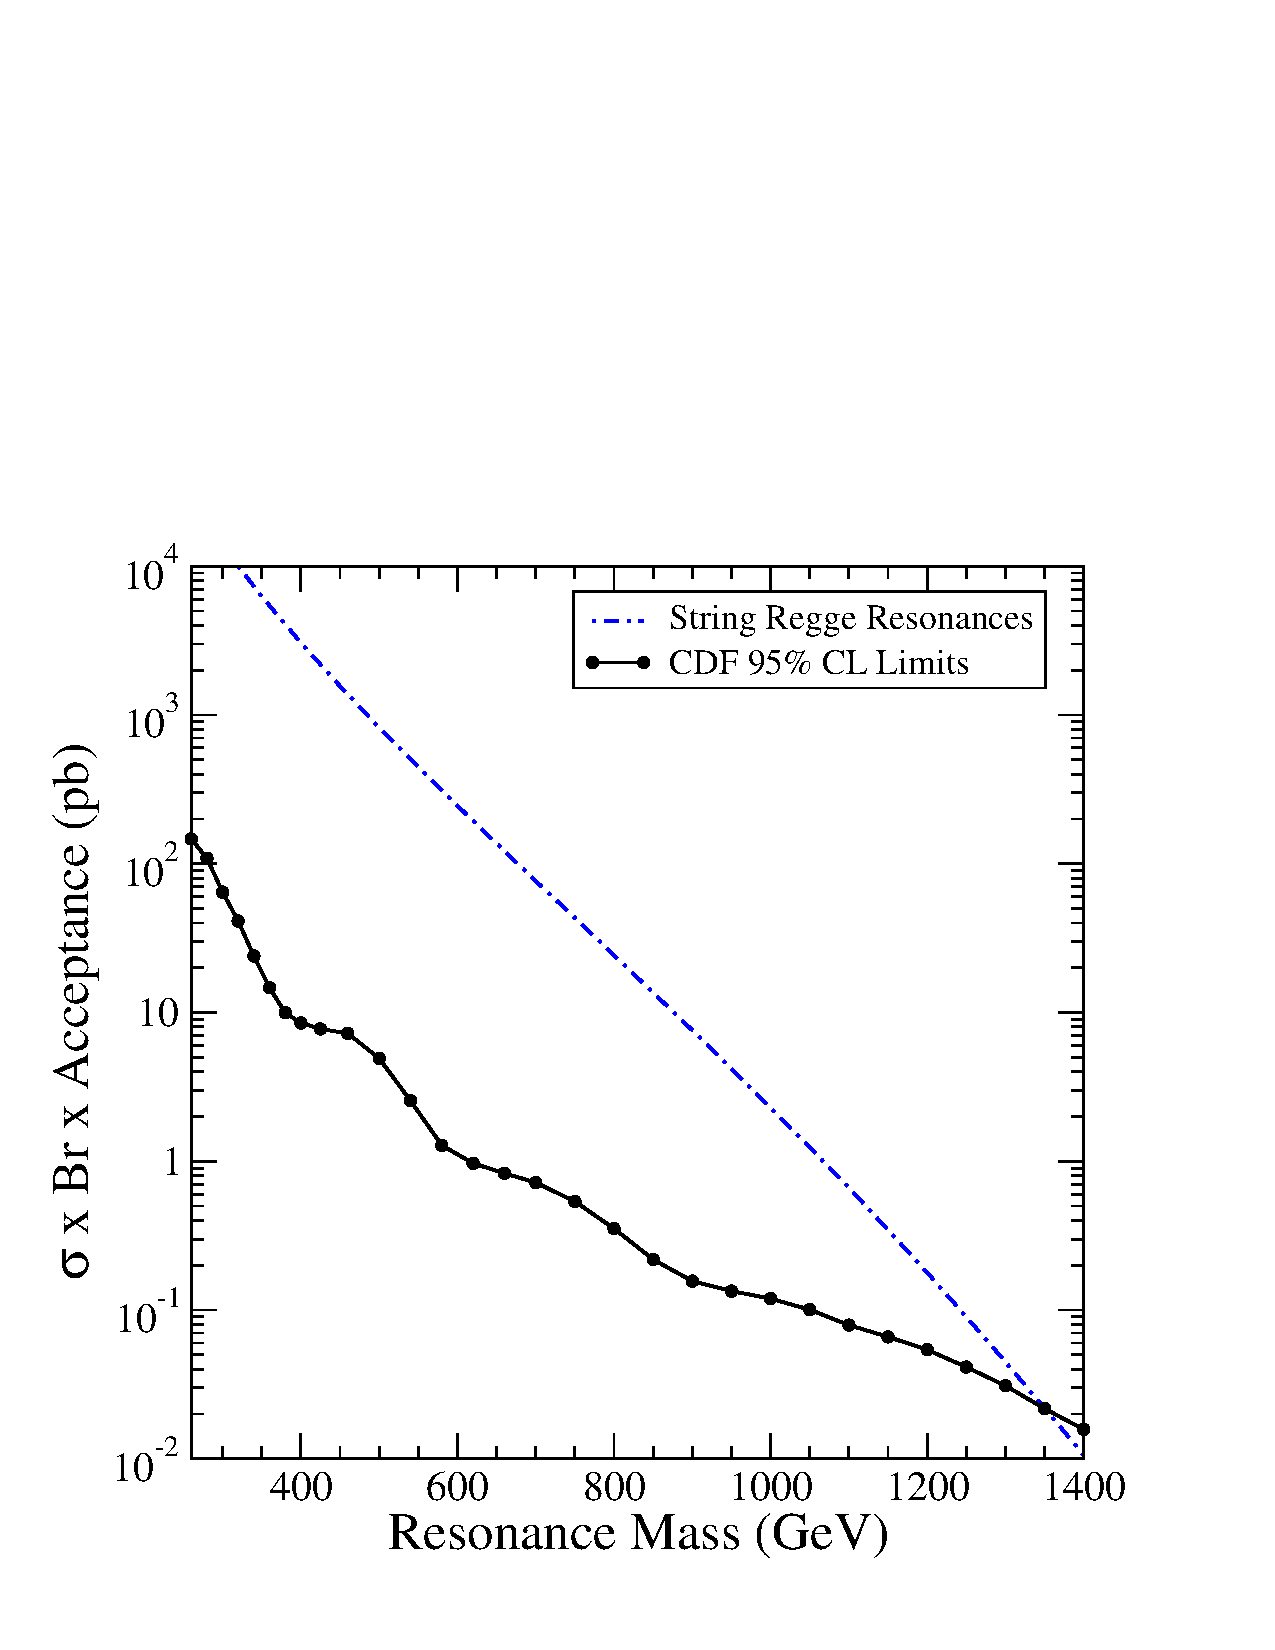
\includegraphics[width=\textwidth]{Figures/CDF_string_exclusion_CMSstyle.pdf}
    \caption{ The 95\% CL upper limits on the cross section for 
    dijet resonances from CDF (points) compared to the predicted cross
    section for string resonances in $p\bar{p}$ collisons at 
    $\sqrt{s}=1.96$ TeV (dash-dot curve).}
    \label{CDFstringLimit}
  \end{center}
\end{figure}

\clearpage
% ----------------------------------------------------------------------------

